\documentclass[a4paper,12pt]{report}
\usepackage[T2A]{fontenc}
\usepackage[utf8]{inputenc}
\usepackage[english,russian]{babel}
\usepackage{graphicx}
\usepackage{wrapfig}
\usepackage{mathtext} 				% русские буквы в фомулах
\usepackage{amsmath,amsfonts,amssymb,amsthm,mathtools} % AMS
\usepackage{icomma} % "Умная" запятая: $0,2$ --- число, $0, 2$ --- перечисление
\usepackage{capt-of}
\usepackage{appendix}
\usepackage{multirow}
\usepackage{hyperref}
\usepackage{floatrow}
\usepackage[left=2cm,right=2cm,
    top=2cm,bottom=2cm,bindingoffset=0cm]{geometry}
\usepackage{multicol} % Несколько колонок
\usepackage{gensymb}
\title{Отчёт по лабораторной работе №77

Операционные усилители}
\author{Плюскова Н.А. Б04-004 }
\date{\today}

\begin{document}

\maketitle

\section*{1. Результаты эксперимента}
\subsection*{1.1 Измерение коэффициента усиление ОУ}

Соберем схему, показанную на рис.\ref{p1}, со следующими параметрами:
\begin{itemize}
    \item $R_{1} = R_{2} = R_{3}$ = 200 кОм
    \item $R_{4}$ = 500 кОм
\end{itemize}

\begin{figure}[H]
    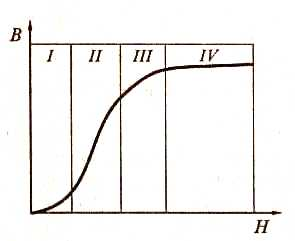
\includegraphics[scale=0.6]{pic1.png}
    \caption{Схема установки к п.1.1 и п. 1.2}
    \label{p1}
\end{figure}

Подадим на вход колебание с амплитудой $U_{in}$ = 3 В и частотой $f$ = 20 Гц:
\begin{itemize}
    \item $U_{a}$ = 12.9 мВ
    \item $U_{out}$ = 564.6 мВ
\end{itemize}

Рассчитаем коэффициент усиления операционного усилителя по формуле:
\begin{equation*}
    A_{0} = (1 + \frac{R_{3}}{R_{4}})\cdot \frac{U_{out}}{U_{a}} = 61.3
\end{equation*}

\subsection*{1.2 Амплитудно-частотная характеристика ОУ}

Для схемы на рис. \ref{p1} снимем зависимость АЧХ, используя формулу:

\begin{equation*}
    A_{0} = (1 + \frac{R_{3}}{R_{4}})\cdot \frac{U_{out}}{U_{a}}
\end{equation*}

Построим полученную зависимость в двойном логарифмическом масштабе:

\begin{figure}[H]
    \includegraphics[scale=0.8]{logA(logf).png}
    \caption{АЧХ операционного усилителя}
    \label{logA(logf)}
\end{figure}

Экстраполируя график до пересечения с уровнями 1 и $A_{0}$, определим граничную частоту $f_{p0}$, соответствующую ослаблению до уровня 0.7 относительно $A_{0}$ и частоту единичного усиления $f_{t}$, на которой коэффициент усиления $A(f) = 1$ (0 дБ):

\begin{itemize}
    \item $f_{p0}$ = 1.8 МГц
    \item $f_{t}$ = 23.5 кГц
\end{itemize}

\subsection*{1.3 Неинвертирующий усилитель}

Собрав схему, изображенную на рис.\ref{p2}, со следующими параметрами:
\begin{itemize}
    \item $R_{1}$ = 90 Ом
    \item $R_{2}$ = 10 кОм
\end{itemize}

\begin{figure}[H]
    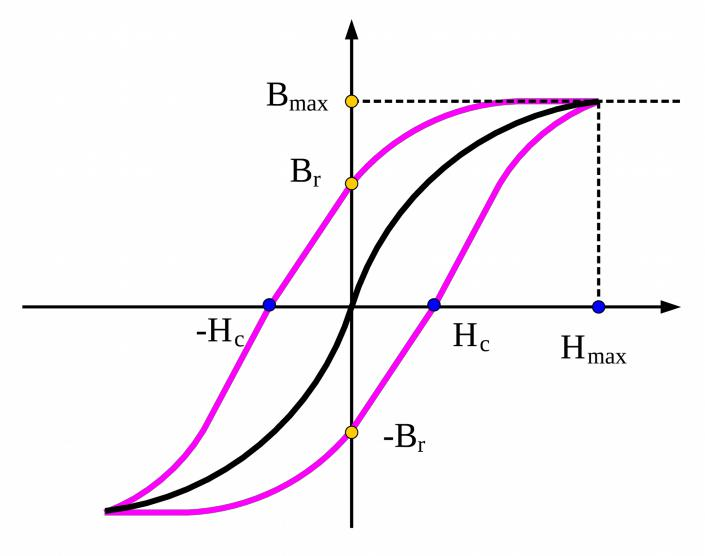
\includegraphics[scale=0.6]{pic2.png}
    \caption{Схема установки к п.1.3}
    \label{p2}
\end{figure}

Определим входное напряжение сдвига: $U_{OS}$ = 19.2 мВ

Снимем зависимость от частоты коэффициента усиления $K(f)$ и построим соответствующий график:

\begin{figure}[H]
    \includegraphics[scale=0.8]{K(f).png}
    \caption{Зависимость $K(f)$}
    \label{logK(logf)}
\end{figure}

Рассчитаем $K_{0}$, $\beta$,$F_{p}$:

\begin{equation*}
    \beta = \frac{R_{1}}{R_{1} + R_{2}} = 0.009
\end{equation*}

\begin{equation*}
    K_{0} = \frac{1}{\beta} = 111 
\end{equation*}

\begin{equation*}
    F_{p} = \beta f_{t} = 28.6  \text{кГц}
\end{equation*}

\subsection*{1.4 Инвертирующий усилитель}

Соберем схему, изображенную на рис.\ref{p3}, со следующими параметрами:
\begin{itemize}
    \item $R_{1}$ = 90 Ом
    \item $R_{2}$ = 10 кОм
\end{itemize}

\begin{figure}[H]
    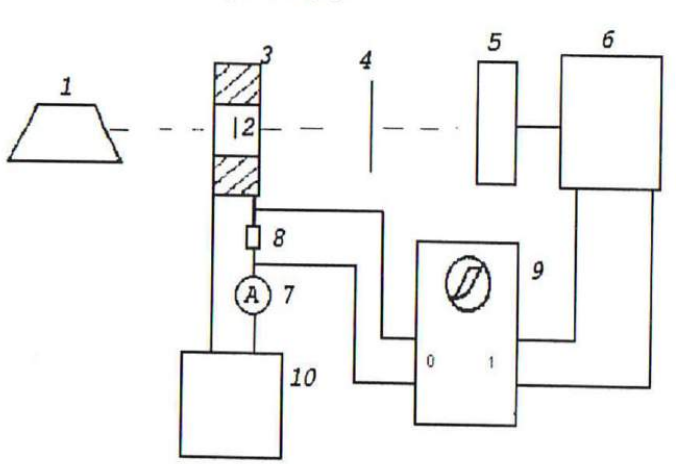
\includegraphics[scale=0.6]{pic3.png}
    \caption{Схема установки к п.1.4}
    \label{p3}
\end{figure}

Определим коэффициент усиления $K_{0}$ и граничную частоту $F_{p}$:
\begin{itemize}
    \item $F_{p}$ = 28.7 кГц
    \item $K_{0}$ = -111 кОм
\end{itemize}

\subsection*{1.5 Интегратор}
Соберем схему, изображенную на рис.\ref{p4}, со следующими параметрами:
\begin{itemize}
    \item $R_{1}$ = 1 кОм
    \item $R_{2}$ = 10 кОм
    \item $C$ = 1 мкФ
\end{itemize}

\begin{figure}[H]
    \includegraphics[scale=0.6]{pic4.png}
    \caption{Схема установки к п.1.5}
    \label{p4}
\end{figure}

Снимем АЧХ интегратора:

\begin{figure}[H]
    \includegraphics[scale=0.8]{logK(logf).png}
    \caption{Зависимость $K(f)$}
    \label{logK(logf)}
\end{figure}

\subsection*{1.6 Триггер Шмитта}
Соберем схему, изображенную на рис.\ref{p5}

\begin{figure}[H]
    \includegraphics[scale=0.6]{pic5.png}
    \caption{Схема установки к п.1.6}
    \label{p5}
\end{figure}

При $U_{ref} = 0$ рассчитаем $\beta$, $R_{1}$ и $R_{2}$:
\begin{itemize}
    \item $R_{1}$ = 1 кОм
    \item $R_{2}$ = 9 кОм
    \item $\beta$ = 0.1
\end{itemize}

Подадим на вход схемы синусоидальное колебание низкой частоты:

\begin{figure}[H]
    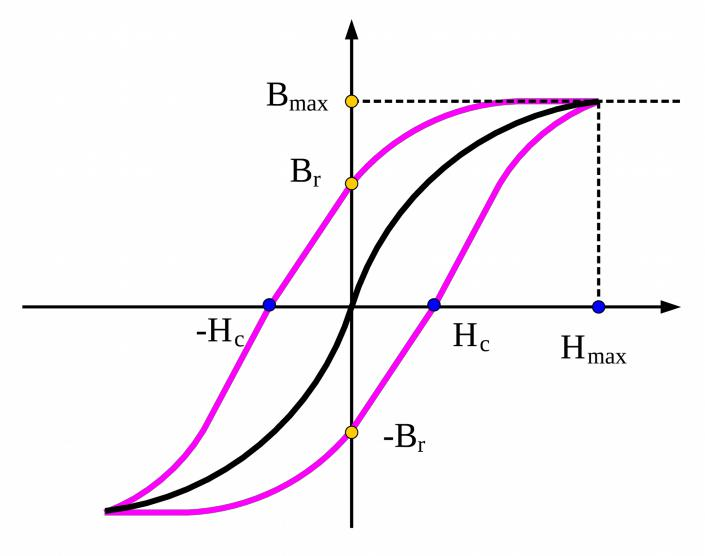
\includegraphics[scale=0.135]{pic2.jpg}
    \caption{Осциллограмма к пункту 1.6}
    \label{pic2}
\end{figure}

При $U_{ref} = 2$В порог срабатывания $U_{\text{порог}} = $ 2.1В

\begin{figure}[H]
    \includegraphics[scale=0.16]{pic4.jpg}
    \caption{Осциллограмма к пункту 1.6}
    \label{pic4}
\end{figure}

\begin{figure}[H]
    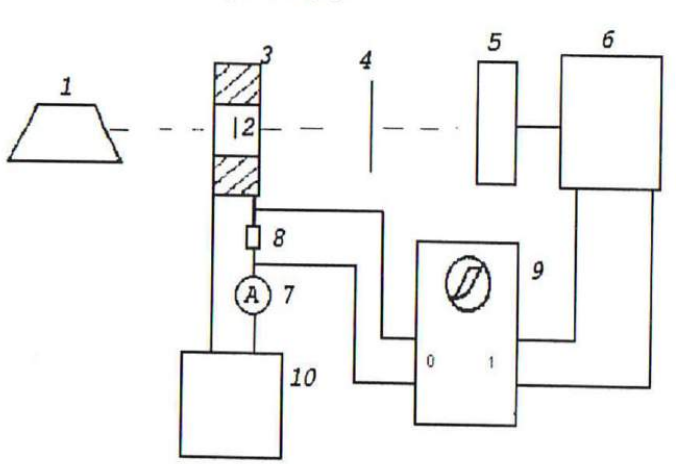
\includegraphics[scale=0.115]{pic3.jpg}
    \caption{Осциллограмма к пункту 1.6}
    \label{pic3}
\end{figure}

\subsection*{1.7 Самовозмуждающийся мультивибратор}
Соберем схему, изображенную на рис.\ref{p6}, со следующими параметрами:
\begin{itemize}
    \item $R_{1}$ = 10 кОм
    \item $R_{2}$ = 90 кОм
    \item $C$ = 0.56 - 0.68 мкФ
    \item $R$ = 4 кОМ
\end{itemize}

\begin{figure}[H]
    \includegraphics[scale=0.6]{pic6.png}
    \caption{Схема установки к п.1.7}
    \label{p6}
\end{figure}

Подадим на вход схемы синусоидальное колебание низкой частоты:

\begin{figure}[h]
    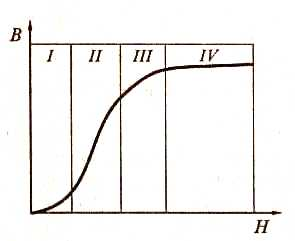
\includegraphics[scale=0.13]{pic1.jpg}
    \caption{Осциллограмма к пункту 1.7}
    \label{pic1}
\end{figure}



\end{document}
